\section{Aufbau und Durchführung}
\label{sec:Durchführung}
Für die Messung der Suszeptibilität wird den Aufbau in der Abbildung \ref{fig:blockschaltbildung} verwendet. Weil es sich um eine Brückenschaltung handelt, tritt das Problem auf, dass es immer eine Störspannung an den Ausgängen gibt, die dann die Brückenspannung komplett überdeckt. Um Störspannung zu vermeiden, wird ein Selektivverstärker verwendet, welcher einerseits nur monofrequente Signalspannungen durchlässt und andererseits die Brückenspannung verstärkt.

\begin{figure}[h!]
	\centering
	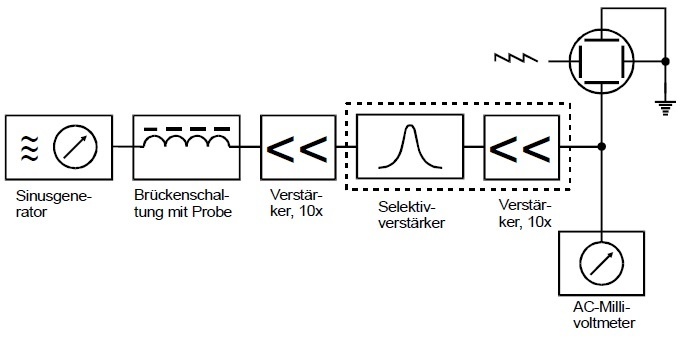
\includegraphics[width=0.9\linewidth]{Blockschaltbildung.jpg}
	\caption{Schematischer Versuchsaufbau mit den Verstärkern, \cite[12]{anleitung606}.}
	\label{fig:blockschaltbildung}
\end{figure}

Es wird ein Linearverstärker genutzt um die Spannungsänderungen meßbar zu machen. Zunächst wird die Filterkurve des Selektivfilters gemessen. Dazu wird die Spannungsquelle direkt mit dem Selektivverstärker verbunden und auf eine feste Spannung und Frequenz eingestellt. 
Die resultierende Ausgangsspannung $U_\text{A}$ bei veränderlicher Spannungsfrequenz wird mit Hilfe von Millivoltmeter abgelesen, gemessen und notiert. Außerdem wird im Bereich von $\SI{25}{\kilo\hertz}$ bis $\SI{30}{\kilo\hertz}$ und von $\SI{40}{\kilo\hertz}$ bis $\SI{35}{\kilo\hertz}$ die zu suchende Frequenz auch gemessen und notiert. Zusätzlich wird die Frequenz in der Nähe des Maximumbereichs in $\SI{0,1}{\kilo\hertz}$ Schritten gemessen und außerhalb in größeren Schritten. 

Im nächsten Versuchsanteil soll nun die Suszeptibilitätsmessung erfolgen. Zuerst wird die Signalfrequenz auf die Durchlassfrequenz des Selektivverstärkers eingeregelt. Die experimentelle Bestimmung erfolgt über zwei Methoden: zum einen über die Änderung der Brückenspannung gegenüber der ohne Probe abgeglichenen Brücke und zum anderen über die Widerstandsdifferenz der abgeglichenen Brücke ohne und mit Probe. Ohne Probe wird die Brückenschaltung mit den beiden Abstimmelementen $\frac{R_3}{R_4}$ und $R_\text{P}$ abgeglichen und danach die beiden Werte aufgeschrieben. Nun wird die Probe in die Spule eingeschoben und erneut die beiden Abstimmelementen notiert. So dann wird noch einmal die Brücke abgeglichen und die neuen sich eingestellten Werte notiert. Das Verfahren wird nun $3$ mal für jeweils $3$ Proben durchgeführt und zwar für: $Nd_2O_3$, $Gd_2O_3$ und $Dy_2O_3$. Pro Probe und Messreihe werden circa $12$ Messwerte aufgeschrieben. Anschließen werden die Länge $l$ und die Masse $m$ der Proben notiert. 